%-----------------------------------------------------------------------------%
\chapter{\babDua}
%-----------------------------------------------------------------------------%
Bab ini akan menjelaskan beberapa teori dan konsep yang perlu dipahami untuk mengerjakan tugs akhir ini. Beberapa diantaranya adalah \iot~, ZigBee, \textit{gateway}, MQTT, dan \textit{social} \iot.

\section{\textit{Internet of Things}}
\textit{\IOT} adalah suatu konsep dimana berbagai macam benda bisa terhubung ke internet. Benda-benda ini bisa bervariasi, mulai dari benda yang memang pada dasarnya sudah bisa terhubung ke internet seperti \textit{smartphone}, hingga benda seperti lampu, kenop pintu,gembok, sensor-sensor, dan berbagai benda lain. Pada konsep ini, selain dapat terhubung ke internet, benda-benda tersebut juga dapat saling berkomunikasi tanpa bantuan manusia, sehingga membentuk suatu jaringan komunikasi antar benda. Implementasi konsep \iot~saat ini sudah sangat beragam, seperti pada bidang \textit{home automation}, bidang kesehatan, bidang retail, dan bidang industri. Beberapa contoh produk populer yang sudah tersedia di pasaran saat ini sebagian besar fokus pada bidang \textit{home automation}, seperti Philips Hue, Nest, WeMo, dan SmartThings.

Istilah \iot~pertama kali disebutkan pada tahun 1999 oleh Kevin Ashton dalam konteks manajemen rantai suplai dengan idenya untuk menggunakan RFID pada barang milik P\&G \cite{AshtonIot}. Ia mengatakan bahwa komputer saat ini hampir seluruhnya bergantung pada manusia untuk mendapatkan informasi seperti melalui data yang diketikkan, mengambil gambar dari pemindai, menekan suatu tombol, dan lainnya. Masalahnya adalah, manusia memiliki waktu, perhatian, dan ketepatan yang terbatas. Bayangkan jika komputer bisa mengetahui segalanya tentang suatu hal tanpa bantuan sama sekali dari manusia. Kita bisa menghitung dan melacak segala hal, dan bisa mengurangi pengeluaran, dan kerugian secara besar-besaran. Kita bisa mencapai hal ini dengan membuat agar sebuah komputer dapat melihat, mendengar, dan membaui lingkungan di sekitarnya dengan sendirinya, tanpa batasan data yang harus dimasukkan oleh manusia\cite{AshtonIot}. Saat ini, istilah \iot~tidak hanya terbatas pada konteks manajemen rantai suplai dan mempunyai kemungkinan implementasi yang lebih luas seperti pada bidang kesehatan, transportasi, pendidikan, manajemen energi, manajemen limbah, layanan publik, dan lainnya.

Saat ini juga sudah ada beberapa definisi mengenai \iot. RFID Group mendefinisikan \iot~sebagai jaringan berskala dunia yang terdiri dari objek yang saling terhubung dan memiliki alamat yang unik berdasarkan protokol komunikasi yang standar\cite{GubbiIot}. Sebuah paper oleh Jayavardhana Gubbi et al.\cite{GubbiIot} juga mendefinisikan \iot~sebagai perangkat yang dapat bergerak dan merasakan keadaan di sekitarnya yang saling terhubung dan dapat berbagi informasi antar berbagai \textit{platform} yang berbeda melalui sebuah framework yang tunggal, yang memberikan gambaran menyeluruh yang dapat membuat munculnya aplikasi inovatif. Hal ini bisa dicapai dengan menggunakan sensor \textit{ubiquitous} yang terus bekerja, analisa data, dan representasi informasi menggunakan \textit{cloud computing}.

Singkatnya, walaupun definisi \textit{'things'} (benda) saat ini sudah berubah, tapi tujuan dari konsep ini menurut Kevin Ashton masih tetap sama, yaitu membuat sebuah mesin agar dapat merasakan apa yang terjadi di sekitar mereka, mengambil informasi dari apa yang terjadi di sekitar mereka, mengolah informasi tersebut, mengirimkannya ke mesin lain, dan kemudian memberikan respons yang sesuai. Semua hal tersebut dilakukan tanpa ada bantuan dari manusia.

\section{\textit{Social} \iot}
\textit{Social} \iot~adalah sebuah konsep yang mencoba menghubungkan konsep \iot~dengan konsep sosial. Terdapat beberapa pendekatan mengenai konsep \siot~ini. Luigi Atzori et al dalam papernya \cite{LuigiSIoT} menawarkan sebuah konsep yang mencoba memberikan hubungan diantara benda-benda, bukan diantara pemiliknya. Hubungan antara benda dengan benda ini meniru hubungan antara manusia dengan manusia. Sebagai contoh, salah satu hubungan yang paling dasar antara manusia adalah hubungan orang tua dengan anak. Dalam papernya, Luigi Atzori et al menamakan hubungan ini sebagai \textit{parental object relationship}, yaitu hubungan antara benda dengan benda lain yang dibuat dalam periode waktu yang sama dan dibuat oleh perusahaan yang sama. Contoh hubungan lain yang ditawarkan dalam paper ini adalah \textit{co-location object relationship} dan \textit{co-work object relationship} seperti yang dilakukan manusia dalam kehidupannya di suatu tempat yang sama atau ketika sedang dalam pekerjaan. Hubungan tersebut ditentukan ketika beberapa benda berada dalam lokasi yang dekat dalam waktu cukup lama atau secara periodik melakukan hubungan untuk melakukan suatu tugas tertentu. Hubungan lain yang cukup menarik yang disebutkan oleh Luigi Atzori et al dalam papernya adalah \textit{social object relationship}. Sama seperti hubungan yang dialami oleh manusia ketika berkenalan dengan manusia lain, pada hubungan ini suatu benda juga dapat bertukar profil sosial dengan benda lain. Melalui hal ini, sebuah benda dapat saling bertukar \textit{best practice} untuk menyelesaikan suatu masalah yang sudah dialami oleh "teman"nya.

Contoh pendekatan lain adalah seperti yang dibuat oleh Dominique Guinard et al \cite{guinard2010sharing}. Dalam papernya, Dominique menawarkan sebuah konsep untuk memanfaatkan hubungan manusia yang terdapat pada layanan sosial media yang sudah ada di pasaran seperti facebook, twitter, dan lainnya. Melalui konsep ini, seorang pengguna dapat membagikan \textit{resource} dari suatu benda yang dimilikinya ke temannya yang terdapat pada suatu media sosial yang sama. Pembagian \textit{resource} ini bisa hanya membagikan status dari \textit{resource} terkait saja (\textit{read only}) atau juga bisa memberikan orang lain akses untuk melakukan kontrol atau merubah status dari benda terkait.

\section{ZigBee}
Zigbee adalah suatu standar yang mendefinisikan sekumpulan protokol komunikasi untuk jaringan nirkabel dengan \textit{data rate} rendah dan jarak yang dekat \cite{farahani2011zigbee}. ZigBee beropeasi di pita frekuensi 868 MHz, 915 MHz, dan 2.4GHz. \textit{Data rate} maksimal dari ZigBee adalah 250 kilo bit per detik.

Walaupun memiliki \textit{data rate} yang rendah, ZigBee memiliki kelebihan dibanding dengan protokol komunikasi lain, yaitu penggunaan daya yang rendah. Hal ini karena memang ZigBee ditargetkan untuk digunakan pada benda yang menggunakan baterai, di mana \textit{data rate} yang dibutuhkan tidak terlalu tinggi, dan biaya yang murah dan daya tahan baterai yang lama adalah kebutuhan utama. Baterai yang digunakan oleh perangkat ZigBee dapat bertahan beberapa tahun sampai perlu diganti. Hal ini dapat dicapai karena pada kebanyakan situasi, total waktu yang digunakan oleh suatu perangkat nirkabel dalam melakukan aktivitas sangat terbatas, sehingga perangkat terkait akan menghabiskan sebagian besar waktunya dalam kondisi hemat daya atau yang dikenal dengan \textit{sleep mode}\cite{farahani2011zigbee}.

Kelebihan lain dari ZigBee adalah topologi jaringannya yang berupa \textit{mesh network}. Ini berarti pengiriman data dari satu perangkat ke perangkat lain bisa tidak dilakukan secara langsung, namun melalui perangkat-perangkat lain sebagai perantara. ZigBee juga memiliki karakteristik \textit{Self-Forming} dan \textit{Self-Healing}. \textit{Self-Forming} berarti sebuah jaringan ZigBee dapat langsung terbentuk ketika perangkat telah aktif tanpa diperlukan supervisi tambahan, sedangkan \textit{Self-Healing} berarti jika salah satu perangkat ZigBee yang berada dalam rute pengiriman data mati karena suatu hal, jaringan ZigBee akan secara otomatis membuat rute pengiriman data yang baru.

Dalam implementasinya, ZigBee memiliki beberapa profil. Profil-profil ini mendefinisikan bagaimana suatu perangkat harus bekerja. Dalam profil ini disebutkan apa saja fungsi-fungsi yang harus ada ketika akan dilakukan implementasi, dan apa saja atribut-atribut yang harus dimiliki oleh suatu perangkat. Dengan mengikuti profil ini, setiap perangkat yang dibuat oleh perusahaan berbeda akan tetap memiliki perilaku yang sama. Beberapa contoh profil yang telah ditentukan adalah:
\begin{itemize}
	\item ZigBee Home Automation 1.2
	\item Light Link 1.0
	\item Building Automation 1.0
	\item Retail Services
	\item Remote Control 2.0
	\item Health Care 1.0
\end{itemize}
Namun pada saat tulisan ini dibuat, ZigBee Alliance sebagai pengembang ZigBee telah mengumumkan versi terbaru dari ZigBee, yaitu ZigBee 3.0. Pada ZigBee versi terbaru ini, dilakukan unifikasi dari berbagai profil ZigBee yang telah disebutkan sebelumnya, sehingga hanya ada satu standar ZigBee. Dengan dilakukannya unifikasi ini, diharapkan dapat memudahkan pengembang perangkat untuk mengembangkan perangkat berbasis ZigBee yang mendukung komunikasi antar perangkat dengan jenis berbeda.

\section{\textit{Gateway}}
\textit{Gateway} adalah sebuah entitas, baik berupa \textit{hardware}, \textit{software}, maupun gabungan keduanya, yang menyalurkan suatu data dari satu tempat ke tempat lainnya. \textit{Gateway} bisa ada dalam banyak bentuk, seperti di antara beberapa LAN, diantara beberapa jenis jaringan yang berbeda, dan juga diantara beberapa aplikasi. \textit{Gateway} biasanya beroperasi di atas \textit{network layer} dan bisa melibatkan semua \textit{layer}. Inti dari sebuah \textit{gateway} adalah konversi atau pengubahan. Sebuah \textit{gateway} akan mengubah pesan yang melewatinya hingga ke \textit{layer} dimana \textit{gateway} tersebut dioperasikan. Tipe \gateway~yang biasa digunakan adalah \textit{application gateway} yang beroperasi di \textit{application layer}. Sebagai contoh, sebuah \gateway~pesan elektronik dapat mengubah pesan dari suatu format pesan elektronik ke format lainnya. \cite{GatewayIbmRedbooks}.

\subsection{ZigBee \Gateway}

Seperti dijelaskan sebelumnya, \textit{gateway} berfungsi sebagai penyalur dan pengubah data yang dikirim dari satu tempat ke tempat lainnya. Berbagai macam \gateway~telah dikembangkan sesuai dengan kebutuhan. ZigBee Alliance sebagai pengembang dari protokol ZigBee juga telah mengeluarkan sebuah standar untuk membuat \gateway. \Gateway~ini dapat digunakan untuk menghubungkan perangkat berbasis ZigBee dengan jaringan lain. Dalam dokumen yang dikeluarkan oleh ZigBee Alliance, dikatakan bahwa perangkat \gateway~ZigBee menyediakan jalur komunikasi menuju sebuah jaringan ZigBee menggunakan IP \textit{based host application} (IPHA) dan sebaliknya dengan menyediakan suatu mekanisme dimana aplikasi eksternal bisa berinteraksi dengan suatu perangkat ZigBee untuk melakukan suatu kontrol atau mengambil suatu data \cite{zigbeegateway}.

ZigBee Alliance juga menyertakan desain arsitektur \gateway~dalam dokumen yang dikeluarkannya. Dalam desain arsitektur tersebut, sebuah \gateway~ZigBee dapat mengimplementasikan satu atau lebih protokol untuk melakukan \textit{Remote Procedure Calls} (RPC). Protokol yang disarankan adalah SOAP, REST, dan GRIP. Pemilihan protokol tersebut dapat dilakukan sesuai kebutuhan pengembang \cite{zigbeeGateway2}. Gambar \ref{fig:arsitektur-zigbee} menunjukkan gambaran arsitektur \gateway~ZigBee yang disediakan oleh ZigBee Alliance.

\begin{figure}
	\centering
	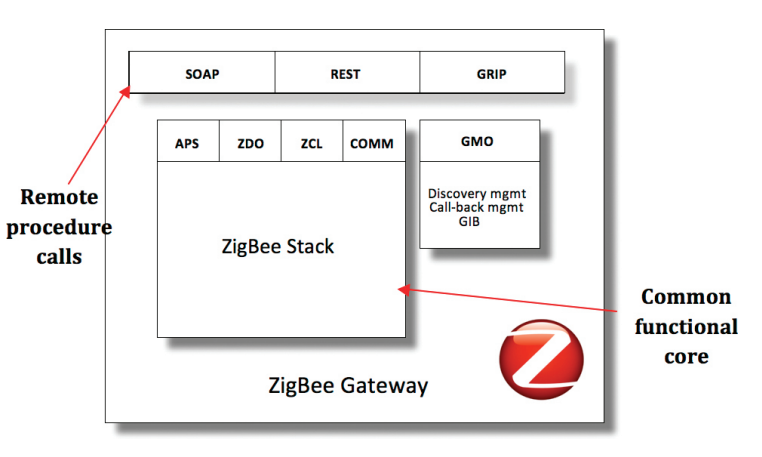
\includegraphics[width=.9\textwidth]{pics/arsitektur-zigbee-gateway.PNG}
	\caption{Arsitektur \Gateway~ZigBee\cite{zigbeeGateway2}}
	\label{fig:arsitektur-zigbee}
\end{figure}

Seperti terlihat pada gambar \ref{fig:arsitektur-zigbee}, implementasi \gateway~ZigBee dibagi menjadi dua lapis. Pada lapisan pertama, terdapat sekumpulan fungsi abstraksi yang tidak tergantung pada protokol dan digunakan untuk melakukan fungsi-fungsi terkait perangkat ZigBee dan pengaturan dari \gateway~itu sendiri. Pada lapisan kedua, terdapat sekumpulan protokol RPC yang dapat digunakan untuk berkomunikasi dengan pihak lain. Untuk pihak lain bisa berkomunikasi dengan \gateway, akan tergantung pada protokol apa yang digunakan pada lapisan kedua ini. \Gateway~kemudian akan mengubah pesan yang diterima di lapisan kedua dan disampaikan kepada lapisan pertama untuk kemudian diproses.

\section{MQTT}
MQTT merupakan singkatan dari \textit{Message Queueing Telemetry Transport}. MQTT adalah sebuah protokol pengiriman pesan yang sangat simpel dan ringan, dan di desain untuk perangkat yang memiliki keterbatasan dan \textit{bandwidth} yang rendah. Hal ini membuat MQTT menjadi cocok untuk kebutuhan komunikasi antar mesin yang tidak memerlukan \textit{bandwidth} yang tinggi namun perlu melakukan komunikasi yang cukup sering dan bisa diandalkan \cite{mqtt.org}.

MQTT di desain agar segala kompleksitas mekanisme pengiriman pesan terdapat di sisi \textit{broker}, sehingga dalam menggunakan \textit{client} MQTT dapat dilakukan dengan mudah. MQTT menggunakan konsep \textit{publish-subscribe} dalam melakukan kerjanya. Model \textit{publish-subscribe} yang digunakan adalah berdasarkan topik. Dengan mengguanakan topik yang disusun menjadi sebuah hirarki, dapat dimungkinkan untuk suatu perangkat melakukan langganan lebih dari satu topik sekaligus \cite{hunkeler2008mqtt}.

\subsection{Sistem \textit{Publish-Subscribe}}

Konsep sistem \textit{publish-subscribe} (pub-sub) adalah suatu model komunikasi dimana pihak yang tertarik untuk mendapatkan informasi mengenai suatu hal, dapat mendaftarkan ketertarikannya. Proses pendaftaran ketertarikan ini disebut proses \textit{subscription}, dan oleh karena itu pihak yang melakukan proses ini disebut \textit{subscriber}. Pihak yang akan memberikan informasi kemudian melakukan suatu proses yang disebut \textit{publishing}, sehingga pihak yang melakukan proses ini disebut sebagai \textit{publisher}. Selain kedua pihak tersebut, perlu ada suat pihak yang berperan menjadi penengah, dan bertanggung jawab untuk mengirimkan dan memastikan informasi yang dikirim oleh \textit{publisher} dapat sampai ke \textit{subscriber}. Pihak yang melakukan pekerjaan ini disebut sebagai \textit{broker} \cite{hunkeler2008mqtt}.

Ada tiga tipe dasar dalam konsep sistem pub-sub ini, yaitu \textit{topic-based} (berdasarkan topik), \textit{type-based} (berdasarkan tipe), dan \textit{content-based} (berdasarkan isi pesan). Pada tipe yang berdasarkan topik, proses \textit{subscription} dan \textit{publishing} hanya dapat dilakukan untuk suatu topik tertentu yang biasanya sudah diketahui terlebih dahulu ketika pengembangan sistem atau aplikasi. Untuk tipe \textit{type-based}, pihak \textit{subscriber} akan memberikan informasi tentang tipe data yang ingin ia \textit{subscribe}, seperti misalnya data penggunaan listrik. Sedangkan untuk tipe yang terakhir yaitu \textit{content-based}, subscriber akan melakukan proses \textit{subscriber} dengan menjelaskan isi pesan seperti apakah yang ingin diterimanya \cite{hunkeler2008mqtt}.

\subsection{Topik dalam MQTT}
Topik dalam MQTT adalah sebuah \textit{string} yang digunakan oleh \textit{broker} MQTT untuk melakukan penyaringan pesan yang akan dikirim kepada \textit{subscriber}. Topik dalam MQTT disusun menjadi suatu hirarki yang terbagi menjadi beberapa level. Setiap level dipisahkan dengan tanda \textit{forward slash} (/). Setiap topik harus memuat minimal satu karakter dan bersifat \textit{case sensitive} \cite{hiveMQtopic}. Gambar \ref{fig:mqtt-topic} menunjukkan contoh topik dalam MQTT.

\begin{figure}
	\centering
	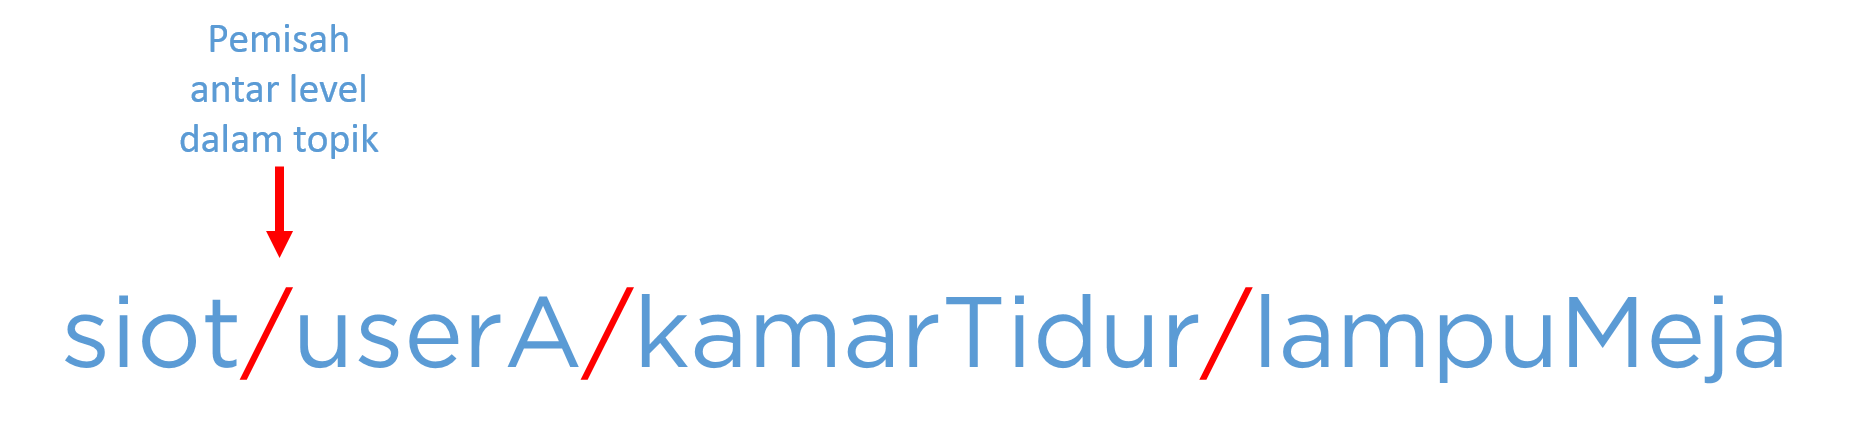
\includegraphics[width=.9\textwidth]{pics/mqtt-topic.PNG}
	\caption{Contoh topik dalam MQTT \cite{hiveMQtopic}}
	\label{fig:mqtt-topic}
\end{figure}

Dalam membuat topik MQTT, kita juga dapat menggunakan \textit{wildcard}. Terdapat dua macam \textit{wildcard} dalam MQTT, yaitu \textit{single level wildcard} yang di tandai dengan karakter tanda tambah (+) dan \textit{multi level wildcard} yang ditandai dengan karakter tanda pagar (\#). \textit{Single level wildcard} dapat digunakan untuk merepresentasikan suatu topik dalam satu level. Gambar \ref{fig:mqtt-single-level-wildcard} menunjukkan contoh penggunaan \textit{single level wildcard}. Sedangkan \textit{multi level wildcard} dapat merepresentasikan lebih dari satu level topik, dan oleh karena itu karakter \textit{multi level wildcard} hanya dapat digunakan sebagai karakter terakhir dalam suatu \textit{string} topik dan harus didahului oleh karakter \textit{forward slash} (/). Namun demikian, kita dapat menggunakan \textit{multi level wildcard} sebagai satu-satunya karakter dalam \textit{string} topik yang berarti \textit{subscriber} akan menerima semua pesan yang dikirimkan ke \textit{broker} \cite{hiveMQtopic}. Gambar \ref{fig:mqtt-multi-level-wildcard} menunjukkan contoh penggunaan \textit{multi level wildcard}.

\begin{figure}
	\centering
	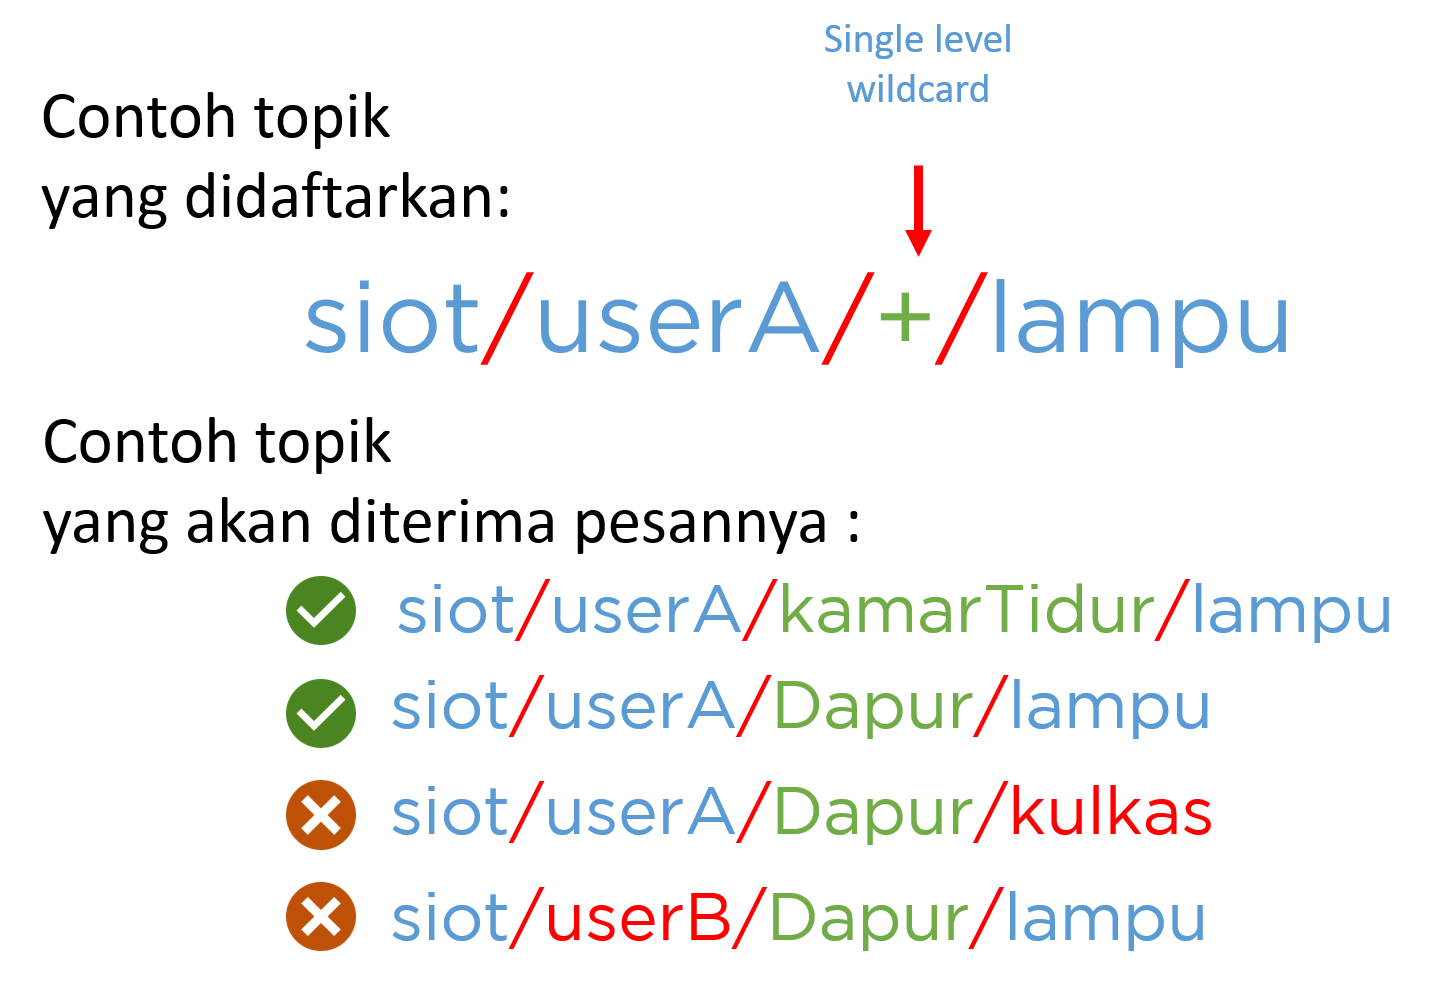
\includegraphics[width=.9\textwidth]{pics/single-level-wildcard.PNG}
	\caption{Contoh \textit{single level wildcard} \cite{hiveMQtopic}}
	\label{fig:mqtt-single-level-wildcard}
\end{figure}

\begin{figure}
	\centering
	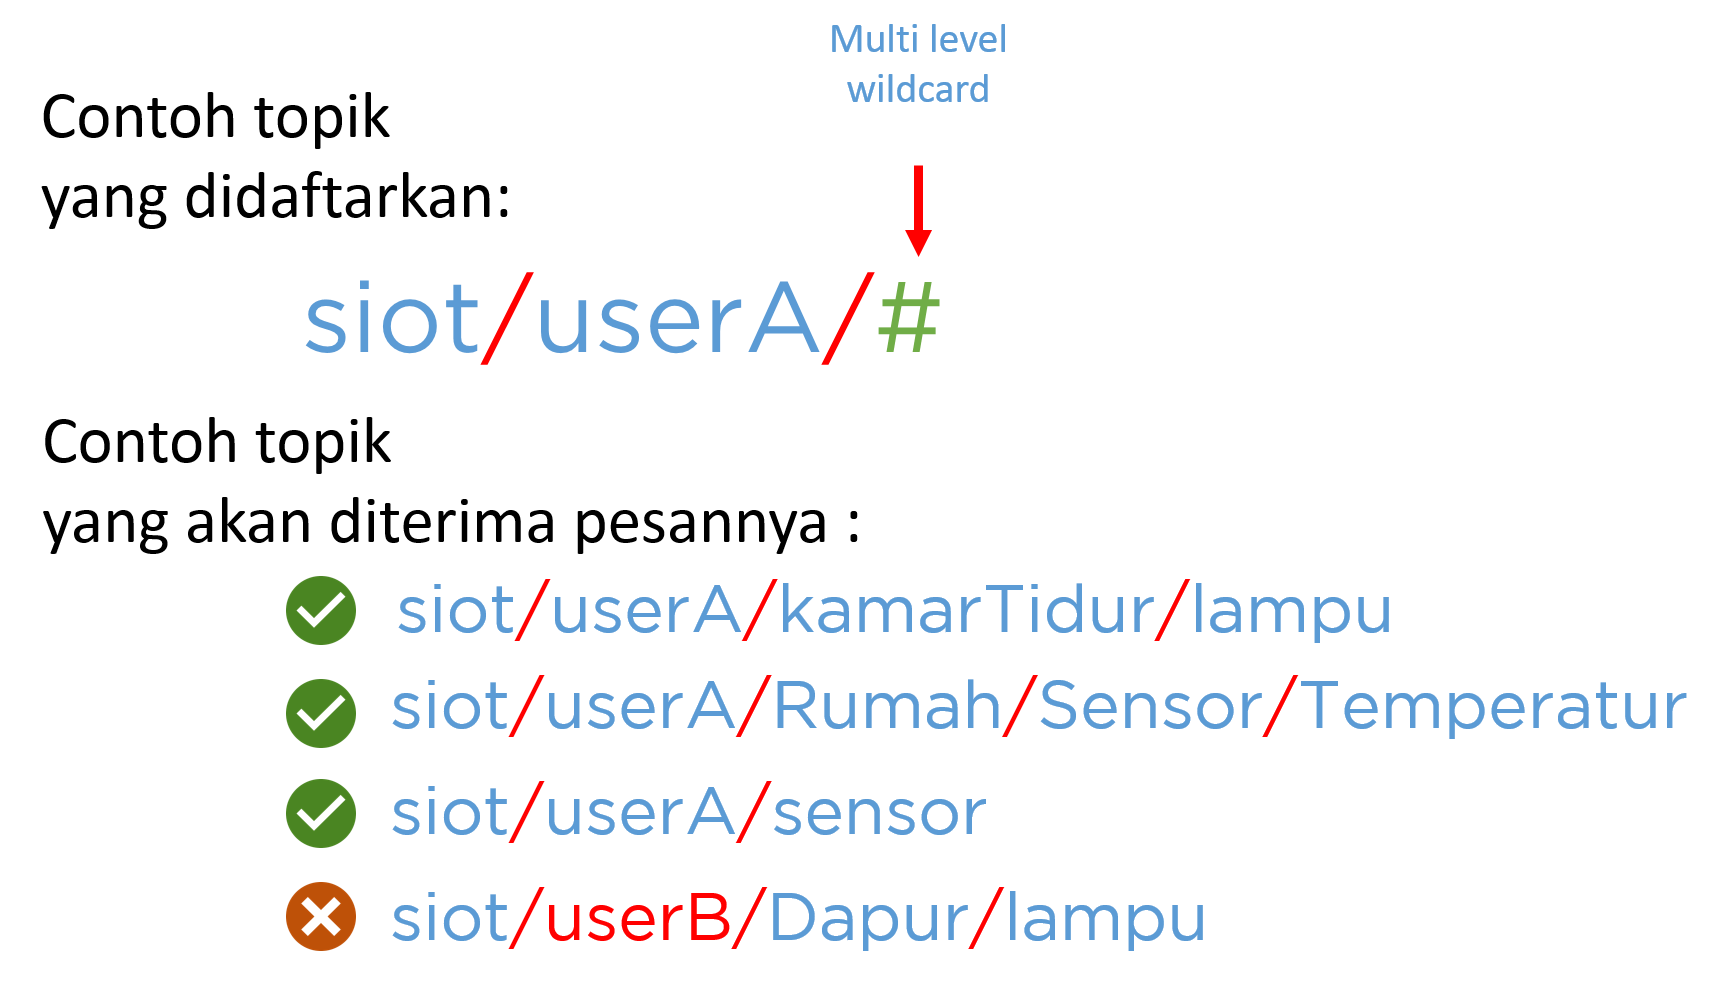
\includegraphics[width=.9\textwidth]{pics/multi-level-wildcard.PNG}
	\caption{Contoh \textit{multi level wildcard} \cite{hiveMQtopic}}
	\label{fig:mqtt-multi-level-wildcard}
\end{figure}
